\chapter{Filters I}

\section{Image representation}
An \textbf{image} is a spatial distribution (two- or three-dimensional) of a physical entity that contains information related to the object (scene) that the image represents. That distribution can be represented as a continuous function that associates, to each point in the plane/space, the intensity of the physical entity at that point $f : \mathbb{R}^{2} \rightarrow \mathbb{R}$(or $f : \mathbb{R}^{3} \rightarrow \mathbb{R}$ for three-dimensional images).\newline
\textbf{Example:}\newline
Let's consider a monochrome image expressible by a continuous function with two independent variables:
\[f(n,m), f: \mathbb{R} \times \mathbb{R} \rightarrow \mathbb{R}\]
\begin{itemize}
    \item \textit{n, m} are the independent spatial coordinates of the image plane
    \item $f(n,m)$ gives the intensities of the measured physical quantity (usually light) at position ($n,m$).
\end{itemize}

\subsection{Digitization}
For digital processing is required a discrete representation of the images. This discretization process is composed by:
\begin{itemize}
    \item \textbf{sampling:} can be expressed as a partition of the image plane in a grid of cells.
    \item \textbf{quantisation:} conversion from the continuous range of values of image intensity to a discrete and finite set of grey values [0-255].
\end{itemize}
\subsection{Digital image representation}
Images can be seen as a Cartesian coordinates system.
\[
    f[n,m] = 
    \begin{bmatrix}
    \ddots & \vdots & \vdots& \vdots & \\
    \dots & f[-1,1] & f[0,1] & f[1,1] & \dots\\
    \dots & f[-1,0] & f[0,0] & f[1,0] & \dots\\
    \dots & f[-1,-1] & f[0,-1] & f[1,-1] &\dots\\
     & \vdots & \vdots & \vdots & \ddots\\
    \end{bmatrix}
\]
where $f[n,m]$ is a \textbf{discrete} function and $n,m$ correspond to rows and columns of a matrix. Each element of the matrix is a \textbf{pixel} and each pixel can have a value, in case of  a grey scale image, between 0-255. By convention, $f[0,0]$ is the center of the image.

\section{Colors}
\subsection{RGB representation}
\begin{center}
    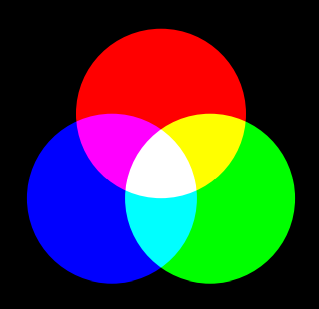
\includegraphics{images/RGB.png}
\end{center}
In the RGB (Red, Green, Blue) system, the primary colors are:
\begin{itemize}
    \item red
    \item green
    \item blue
\end{itemize}
By composing two primary colors, you obtain secondary colors:
\begin{itemize}
    \item cyan = green + blue
    \item magenta = red + blue
    \item yellow = red + green
\end{itemize}
By composing all the primary colors, you obtain white.\newline
An RGB-encoded image consists of three channels, one for each component, where each color is obtained mixing red, green and blue values. If you use 8 bit to represent each component, the number of distinct colors that can be represented in the image is $(2^{8})^{3} = 16 777 219$.\newline
The function that describes an RGB-image is the following:
$$f[n,m] = \left[
\begin{array}{c}
r[n,m]\\
g[n,m]\\
b[n,m]
\end{array}\right]
$$

\subsection{HSV representation}
\begin{center}
    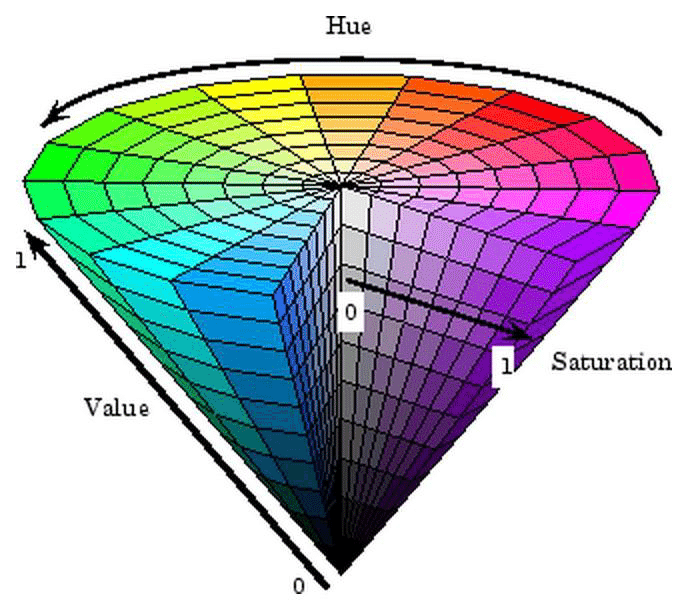
\includegraphics[scale = 0.3]{images/HSV.png}
\end{center}
The HSV representation specifies colors in term of:
\begin{itemize}
    \item \textbf{hue:} dominant color
    \item \textbf{saturation:} it measures how far you are from the fully saturated color (in which you don't have any grey).
    \item \textbf{lightness:} color brightness. While saturation measures the “dilution” of hue with white, brightness indicates dilution with black.
\end{itemize}
HSV representation is closer to how people perceive colors.

\section{Histogram of an image}
The histogram of an image associates to each grey (or RGB) level the number of pixels in which it occurs (i.e. its frequency). So it represents the global distribution of grey (or RGB) levels in a given image.
\begin{flushleft}
    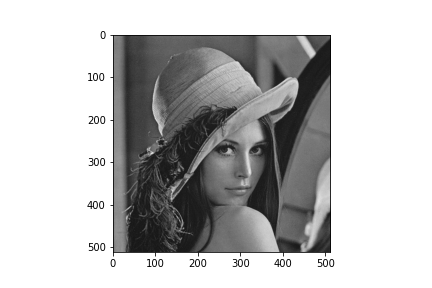
\includegraphics[scale=0.5]{images/lena GS.png}
    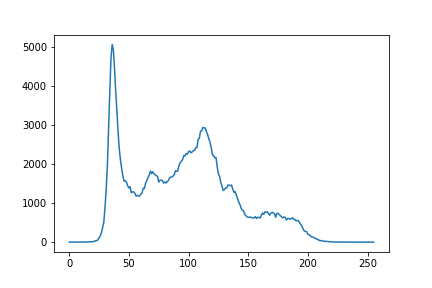
\includegraphics[scale=0.5]{images/histogram GS.png}
    
    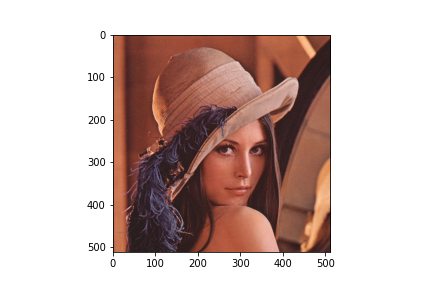
\includegraphics[scale=0.5]{images/lena RGB.png}
    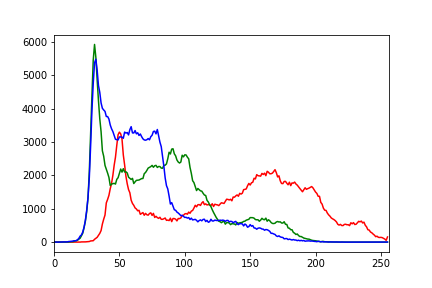
\includegraphics[scale=0.5]{images/histrogram RGB.png}
\end{flushleft}
Histograms are very simple image representation and they are not robust at all against any image transformation (e.g. changing in illumination).

\section{Filters}
\textbf{Filtering:} Forming a new image whose pixel values are transformed from the original ones.\newline
The goals of filtering are:
\begin{itemize}
    \item \textbf{extract} useful information
    \item \textbf{transform} images into another domain where we can modify/enhance image properties.
\end{itemize}
\subsection{Linear Filters}
We define a filter as a unit that converts an input function $f[n,m]$ into an output function $g[n,m]$, where ($n,m$) are the independent variables. \newline
Linear filters work by moving a sliding window (kernel) through the image, pixel by pixel. The window contains coefficients which characterize the transformation. At each position, the result of the filter is calculated by combining the values of the image subtended to the window with the coefficients of the window itself. In order to compute the new value of the central pixel, the coefficients are:
\begin{itemize}
    \item multiplied by the values of the original image subtended to the window
    \item added
\end{itemize}
These filters are defined by the following mathematical operator called \textbf{convolution}:
\[(f * h)[n,m] = \sum_{k,l}f[k,l]h[n-k, m-l]\]
where $h$ is the \textit{kernel}.\newline
Note that the kernel must have an odd number of rows and columns, because it is centered on the pixel to process.\newline \newline
\textbf{Borders:}\newline
Given an $n \times n$ kernel, its external row/column coincides with the border of the image when the center of this mask is at distance $\frac{n-1}{2}$ from the edge. If you move further out, part of the window \textit{leaves} the image.\newline
This situation can be managed in three different ways:
\begin{itemize}
    \item limit the movement of the mask, keeping it at a minimum distance of $\frac{n-1}{2}$ from the edges.
    \item duplicate the external rows/columns of the image
    \item enlarge the image with rows/columns of zeros
\end{itemize}
Solution 1 gives reliable results, but produces a different size image from the original. Solutions 2 and 3, on the other hand, give results that are not exactly authentic near the edges, but are often convenient because they allow you to obtain an output image with the same size as the input one.

\subsection{Smoothing filters}
Smoothing filters are low-pass filters: they emphasize low frequencies and attenuate the high frequencies. They cause image blur, which is helpful to:
\begin{itemize}
    \item remove small details
    \item reduce noise in the image
\end{itemize}
\textbf{Examples:}
\begin{itemize}
    \item \textbf{Moving average filter} (\textit{box filter}) in which all the kernel coefficients are equal to 1.
    \begin{center}
        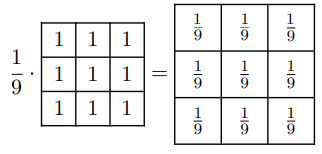
\includegraphics[]{images/box filter.png}
    \end{center}
    It is defined by the following formula:
    \[g[n,m] = \frac{1}{9}\sum_{k=-1}^{1}\sum_{l=-1}^{1}f[n-k, m-l]\]
    Basically, it replaces each pixel with an average of its neighbors. This filter can be applied in order to remove small details, to obtain blurring effect (more evident as the size of the window increases) but it is not useful to remove the so called \textit{salt and pepper noise}, because corrupted pixels affect the computation of the average, so the noise points can even tend to dilate.
    
    \item \textbf{Gaussian Filter} is a weighted average filter with coefficients derived from two-dimensional Gaussian function.
    \begin{center}
        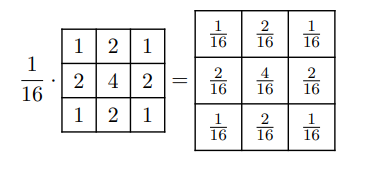
\includegraphics[]{images/gaussian filter.png}
    \end{center}
    where 16 is the sum of the kernel coefficients\newline
    The one-dimensional Gaussian with mean $\mu$ and standard deviation $\sigma$ has the following shape:
    \[G(x) = \frac{1}{\sigma \sqrt{2\pi}}e^{-\frac{(x-\mu)^{2}}{2\sigma^{2}}}\]
    \begin{center}
        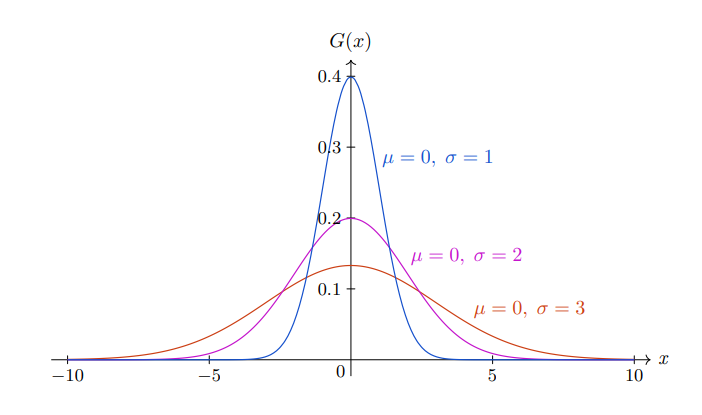
\includegraphics[]{images/Gaussian.png}
    \end{center}
    The kernel is an approximation of a 2D Gaussian function in which pixels near the center of the window have more weight than the outer ones
    \[\frac{1}{2\pi \sigma^{2}}e^{-\frac{u^{2} + v^{2}}{2\sigma^{2}}}\]
    Like the box-filter presented above, it removes high-frequency components and produces blurring effect.\newline\newline
    The filter has two main parameters:
    \begin{itemize}
        \item \textbf{size of the kernel}: A bigger kernel approximates better the Gaussian function, but it increases the computational cost of the filtering process
        \item \textbf{variance} $\sigma$: It determines the extent of smoothing. Increasing the value of $\sigma$ means to increase the blurring effect. In fact, as sigma increases, the weights of the pixels near the center decrease and the weights of the outer pixels increase.
    \end{itemize}
\end{itemize}
Note that, for this kind of filters, the sum of the window's values has to be equal to one, because constant regions shouldn't be affected by the application of the filter
\subsection{Median filter}
The median filter is not a convolutive operator. In fact, it uses an "empty" window, with no coefficients: it replaces each pixel of the input image with the \textbf{median} of its neighborhood. This filter is effective in reducing \textit{salt and pepper noise}, because the presence of any corrupted pixel does not influence the result (unless these pixels are particularly numerous in a certain neighbourhood). Also, it does not degrade too much the edges of the image.

